\documentclass[tikz,border=10pt]{standalone}
\usepackage{lmodern}        % Latin Modern fonts - prevents font warnings
\usepackage[T1]{fontenc}    % Proper font encoding
\usepackage{tikz}
\usepackage{xcolor}
\usetikzlibrary{shapes.geometric,arrows.meta,positioning,fit,patterns,calc}

\definecolor{userspace}{RGB}{173,216,230}
\definecolor{kernelspace}{RGB}{255,165,79}
\definecolor{unused}{RGB}{220,220,220}

\begin{document}
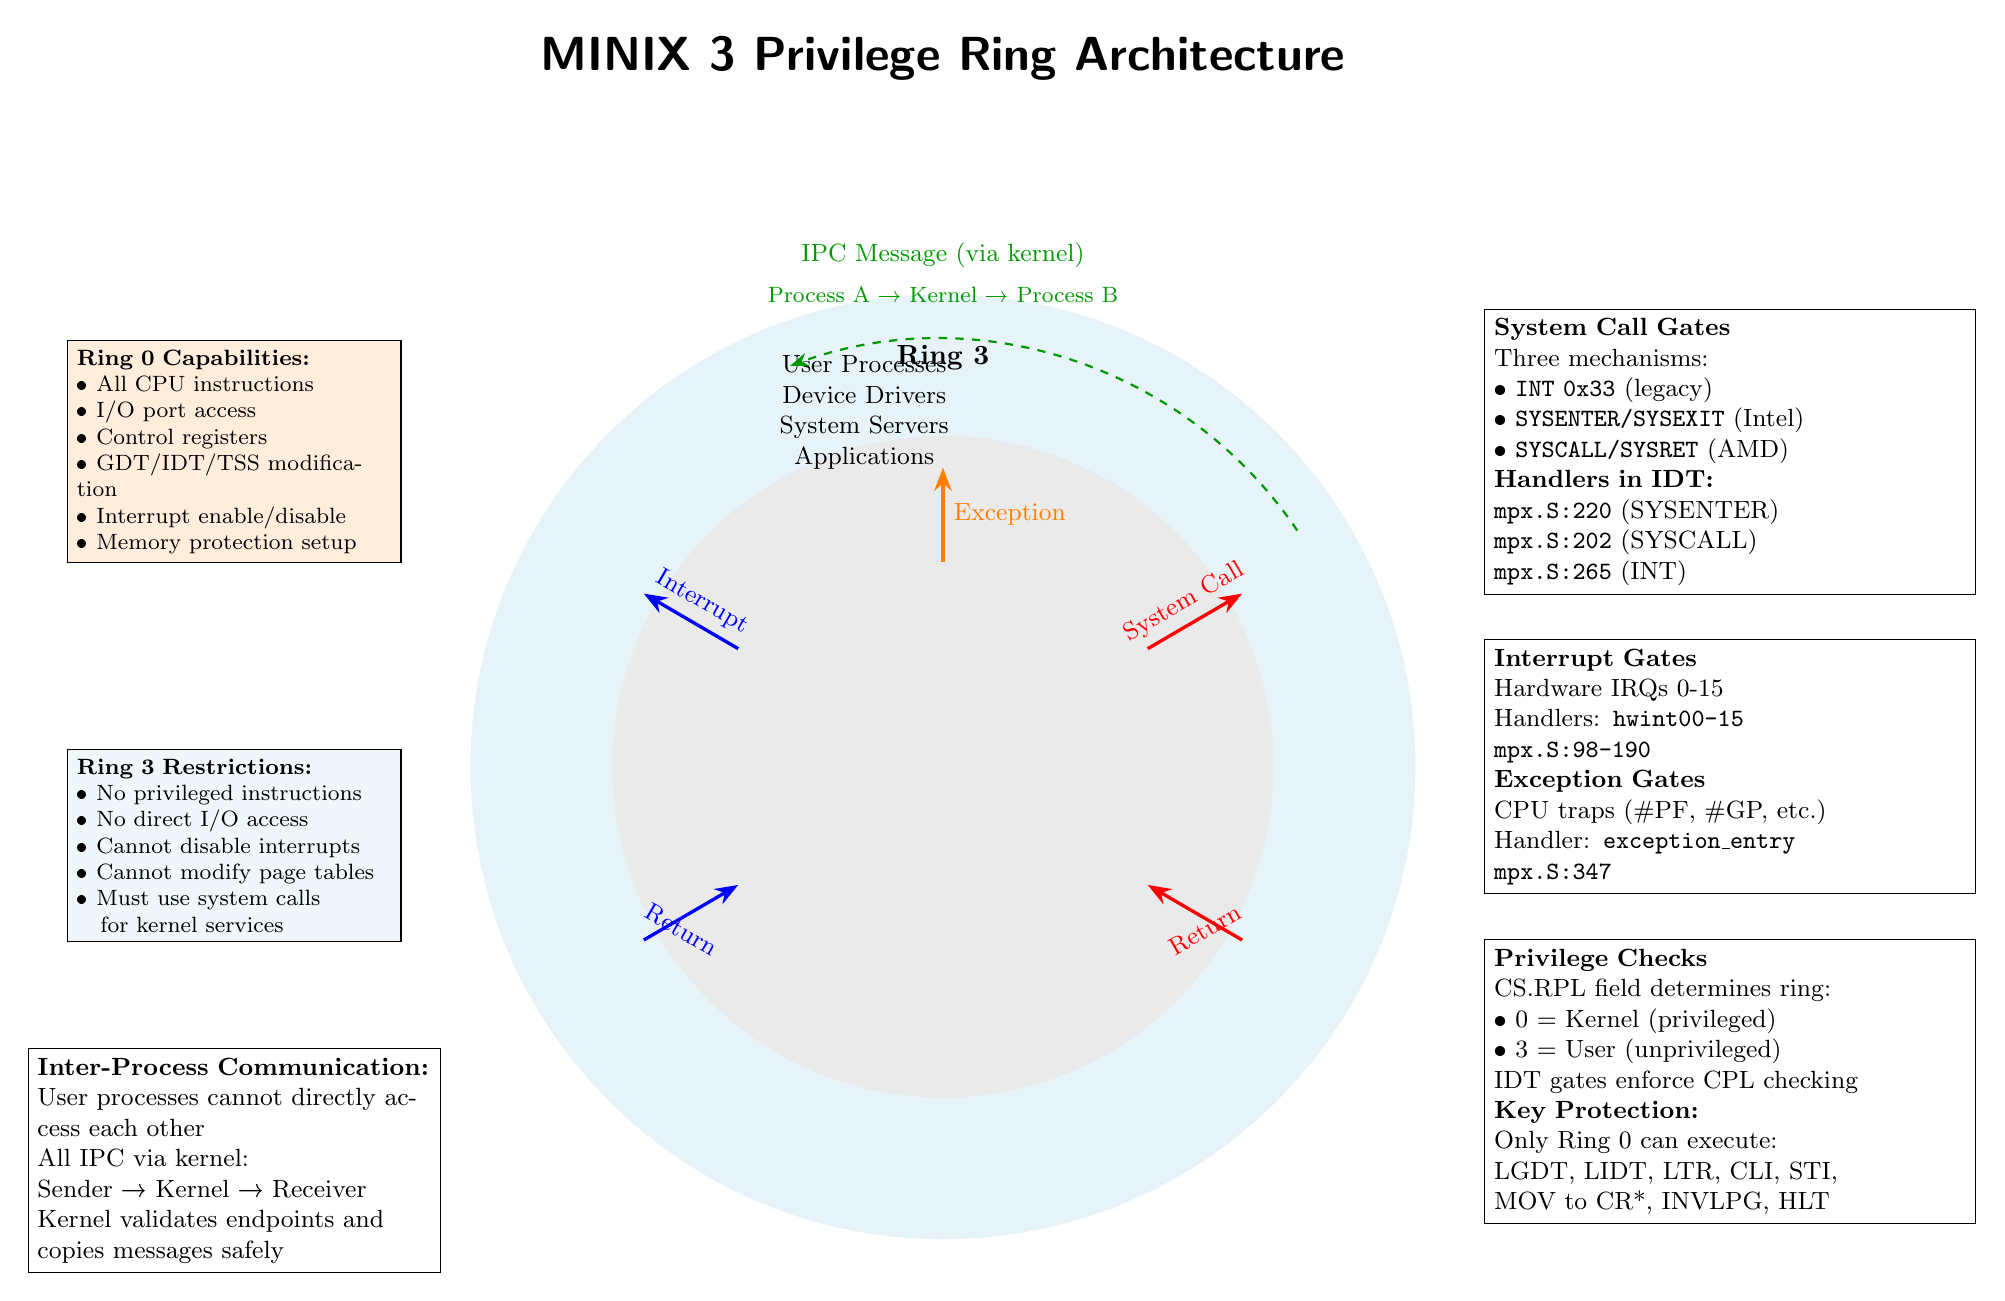
\begin{tikzpicture}[
    every node/.style={font=\sffamily},
    arrow/.style={-Stealth, very thick},
]

% Title
\node[font=\sffamily\LARGE\bfseries] at (0, 9) {MINIX 3 Privilege Ring Architecture};

% Ring 0 (innermost) - Kernel
\fill[kernelspace!40] (0,0) circle (2.5cm);
\node[text width=4cm, align=center, font=\bfseries] at (0,0.5) {Ring 0};
\node[text width=4cm, align=center, font=\small\bfseries] at (0,0) {Microkernel Core};
\node[text width=4.5cm, align=left, font=\ttfamily\footnotesize] at (0,-0.8) {
    mpx.S\\
    klib.S\\
    proc.c\\
    protect.c\\
    system.c
};

% Ring 1 & 2 (not used) - Gray band
\fill[unused!60] (0,0) circle (4.2cm);
\fill[kernelspace!40] (0,0) circle (2.5cm);

\node[text width=3cm, align=center, font=\bfseries] at (0,3.2) {Rings 1 \& 2};
\node[text width=3cm, align=center, font=\small] at (0,2.8) {UNUSED};
\node[text width=4cm, align=center, font=\footnotesize, text=gray] at (0,2.4) {(Not used by MINIX)};

% Ring 3 (outermost) - User space
\fill[userspace!30] (0,0) circle (6cm);
\fill[unused!60] (0,0) circle (4.2cm);

\node[text width=3cm, align=center, font=\bfseries] at (0,5.2) {Ring 3};
\node[text width=5cm, align=center, font=\small] at (-1,4.5) {
    User Processes\\
    Device Drivers\\
    System Servers\\
    Applications
};

% Gates (arrows showing transitions)
% System call gate
\draw[arrow, color=red] (2.6, 1.5) -- (3.8, 2.2) node[midway, above, font=\small, rotate=30] {System Call};
\draw[arrow, color=red] (3.8, -2.2) -- (2.6, -1.5) node[midway, below, font=\small, rotate=30] {Return};

% Interrupt gate
\draw[arrow, color=blue] (-2.6, 1.5) -- (-3.8, 2.2) node[midway, above, font=\small, rotate=-30] {Interrupt};
\draw[arrow, color=blue] (-3.8, -2.2) -- (-2.6, -1.5) node[midway, below, font=\small, rotate=-30] {Return};

% Exception gate
\draw[arrow, color=orange] (0, 2.6) -- (0, 3.8) node[midway, right, font=\small] {Exception};

% IPC flow annotation (Ring 3 to Ring 3 via Ring 0)
\draw[arrow, dashed, thick, color=green!60!black] (4.5, 3) arc (34:110:5.5cm);
\node[font=\small, text=green!60!black] at (0, 6.5) {IPC Message (via kernel)};
\node[font=\footnotesize, text=green!60!black] at (0, 6) {Process A → Kernel → Process B};

% Legend boxes
\node[draw, fill=white, text width=6cm, align=left, font=\small] at (10, 4) {
    \textbf{System Call Gates}

    Three mechanisms:

    • \texttt{INT 0x33} (legacy)

    • \texttt{SYSENTER/SYSEXIT} (Intel)

    • \texttt{SYSCALL/SYSRET} (AMD)

    \textbf{Handlers in IDT:}

    \texttt{mpx.S:220} (SYSENTER)

    \texttt{mpx.S:202} (SYSCALL)

    \texttt{mpx.S:265} (INT)
};

\node[draw, fill=white, text width=6cm, align=left, font=\small] at (10, 0) {
    \textbf{Interrupt Gates}

    Hardware IRQs 0-15

    Handlers: \texttt{hwint00-15}

    \texttt{mpx.S:98-190}

    \textbf{Exception Gates}

    CPU traps (\#PF, \#GP, etc.)

    Handler: \texttt{exception\_entry}

    \texttt{mpx.S:347}
};

\node[draw, fill=white, text width=6cm, align=left, font=\small] at (10, -4) {
    \textbf{Privilege Checks}

    CS.RPL field determines ring:

    • 0 = Kernel (privileged)

    • 3 = User (unprivileged)

    IDT gates enforce CPL checking

    \textbf{Key Protection:}

    Only Ring 0 can execute:

    LGDT, LIDT, LTR, CLI, STI,

    MOV to CR*, INVLPG, HLT
};

% Annotation showing what each ring can do
\node[draw, fill=kernelspace!20, text width=4cm, align=left, font=\footnotesize] at (-9, 4) {
    \textbf{Ring 0 Capabilities:}

    • All CPU instructions

    • I/O port access

    • Control registers

    • GDT/IDT/TSS modification

    • Interrupt enable/disable

    • Memory protection setup
};

\node[draw, fill=userspace!20, text width=4cm, align=left, font=\footnotesize] at (-9, -1) {
    \textbf{Ring 3 Restrictions:}

    • No privileged instructions

    • No direct I/O access

    • Cannot disable interrupts

    • Cannot modify page tables

    • Must use system calls

    \quad for kernel services
};

% Title for IPC
\node[draw, fill=white, text width=5cm, align=left, font=\small] at (-9, -5) {
    \textbf{Inter-Process Communication:}

    User processes cannot directly access each other

    All IPC via kernel:

    Sender → Kernel → Receiver

    Kernel validates endpoints and copies messages safely
};

\end{tikzpicture}
\end{document}
